\chapter{M2Go Part 2: Golang}
\label{cha:golang}
This section introduces the Golang programming language.
It is a compiled, statically typed language developed by Google, commonly used for network and web applications.
Its performance and simplicity make it a good choice for microservices, APIs and other network applications.

The first section is about setting up the Golang environment and cloning the GitLab repository.
\autoref{sec:basic_go_program} will introduce the basic syntax of Golang by implementing a simple hello world program.
\autoref{sec:go_program_car_rental} will manifest the basic Golang knowledge by analyzing the structure and requirements of the CarRental program.
Finally, \autoref{sec:advanced_go_program_car_rental_cli} will introduce advanced Golang features by implementing a command line interface for the CarRental program.

%==============================================================================

\section{M2Go Environment Installation}
\label{sec:m2go_env_installation}
This section provides an overview of the M2Go environment, the installation and the usage of the GitLab instance.
\label{sec:exercise_install_go_env}

\subsection{Exercise M2GoEnvironmentInstallation}
\label{sec:exercise_m2go_environment_installation}

\subsubsection*{Environment Description}
The hardware used is a Windows Surface Studio with an 11th Gen Intel Core i5-11300H, 16 GB of RAM, and 256 GB of SSD storage.
The operating system is Windows 11 64-bit. However, the installation is carried out on WSL 2 running Ubuntu 20.04.6 LTS installed on the machine.

\subsubsection*{Installation Steps}
WSL2 (Ubuntu 20.04.6 LTS), VSCode (1.84.2) and Git (2.25.1) are already installed on the machine. 
Therefore no further installation steps are required for these tools.
The correct environment-installation on the author's machine can be seen in \autoref{fig:screendump_installation}.

Carrying out the installation of Go, version go1.21.4 is installed.
To install Go on the machine, the following steps are required:
\begin{enumerate}
    \item Download the latest version of Go from \url{https://go.dev/dl/go1.21.4.linux-386.tar.gz} by using  \texttt{wget} in the terminal.
    \item Extract the downloaded archive to \texttt{/usr/local} via \texttt{sudo tar -C /usr/local -xzf go1.21.3.linux-386.tar.gz}
    \item Under \texttt{/etc/profile} add the following lines to the bottom of the file: 
    \begin{itemize}
        \item \texttt{export PATH=\$PATH:/usr/local/go/bin}
        \item export \texttt{GOPATH=\$HOME/go}
    \end{itemize}
    \item Now reload the terminal or force the update by running \texttt{source \$HOME/.profile}
    \item Verify the installation by running \texttt{go version}
\end{enumerate}

\begin{figure}[H]
	\centering
	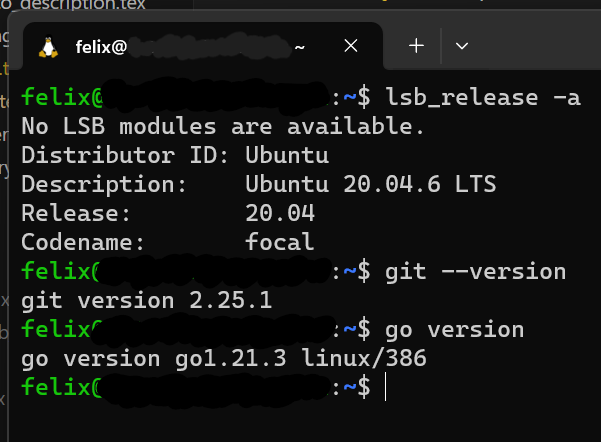
\includegraphics[width=0.5\textwidth]{figures/goLang/installation_screendump.png}
	\caption{Screendump showing the correct installation of the environment}
	\label{fig:screendump_installation}
\end{figure}

Further details on the installation and especially the path variables can be found in \autoref{sec:go_environment_variables} on path variables in Ubuntu.
\label{sec:exercise_cm_gitlab_usage}

\subsection{Exercise CMGitLabUsage}

\subsubsection*{Description of the M2Go Subgroup Structure}
The subgroup structure in \autoref{fig:screendump_subgroupStructure} only contains the Golang repository.
As the course advances, more repositories will be added to this subgroup.
This repository consists of the following three folders:
\begin{enumerate}
    \item BasicGoProgram/HelloWorld: This folder contains the hello world program introducing the basic Golang syntax
    \item CarRental: This folder contains the CarRental program introducing general Golang features
    \item CarRentalCLI: This folder contains the CarRentalCLI program implementing a more complex version of the CarRental program
\end{enumerate}
Furthermore, there is the .gitignore file and the README.md file.
This structure can be further examined in \autoref{fig:screendump_subsubgroupStructure}.

\begin{figure}[h]
    \centering
    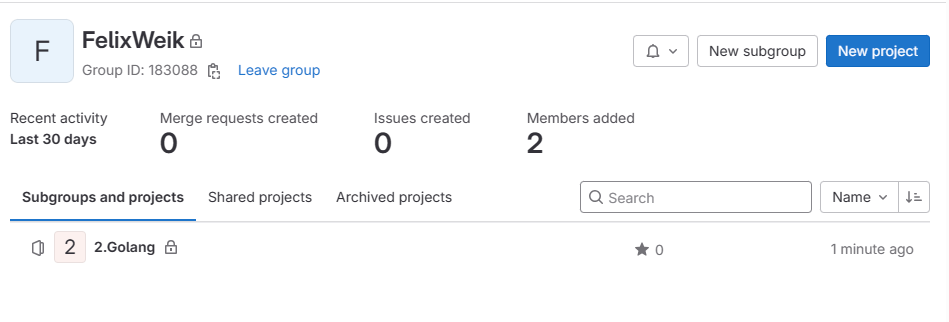
\includegraphics[width=0.8\textwidth]{figures/goLang/golang_personalSubgroupStructure.png}
    \caption{Screendump showing the Subgroup Structure}
    \label{fig:screendump_subgroupStructure}
\end{figure}

\begin{figure}
    \centering
    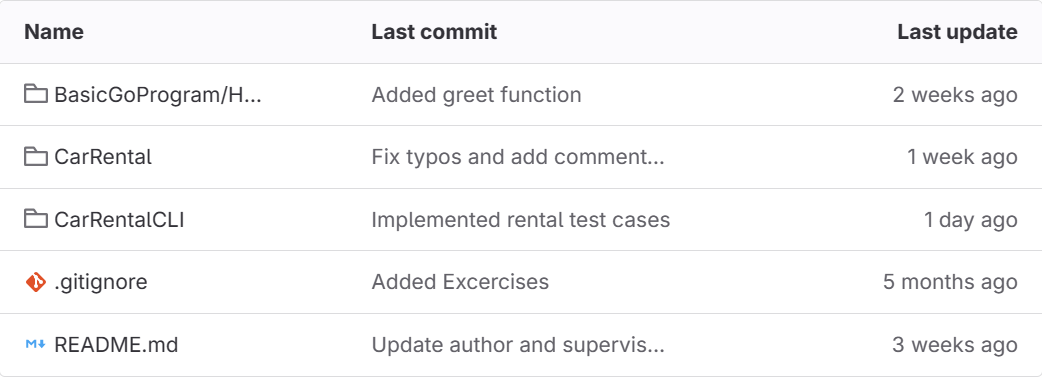
\includegraphics[width=0.8\textwidth]{figures/goLang/golang_personalSubsubgroupStructure.png}
    \caption{Screendump showing the Subgroup Structure of the Golang Folder}
    \label{fig:screendump_subsubgroupStructure}
\end{figure}

\subsubsection*{Repository Cloning Steps}
To clone the repository, the following steps are required:
\begin{enumerate}
    \item Create a Personal Access Token (PAT) on GitLab by going to your Profile Settings and then to Access Tokens
    \item Save the PAT in a safe place
    \item Go to the repository and copy the HTTPS clone URL
    \item Open the WSL2 terminal and navigate to the folder where you want to clone the repository, in the author's case \texttt{/home/felix/WASA\_M2Go}
    \item Download the repository by running the following command in the terminal: \texttt{git clone <HTTPS clone URL>}
\end{enumerate}

\subsubsection*{First Commit}
After changing the placeholder text in the README.md file, the first commit is done by using the graphical features Visual Studio Code offers.
The commit message shown in \autoref{fig:screendump_readmeCommitMessage} is the following: \texttt{Update author and supervisor in README.md}.

After committing the changes, the changes are pushed to the remote repository, which then becomes visible as shown in \autoref{fig:screendump_readme}.

\begin{figure}
    \centering
    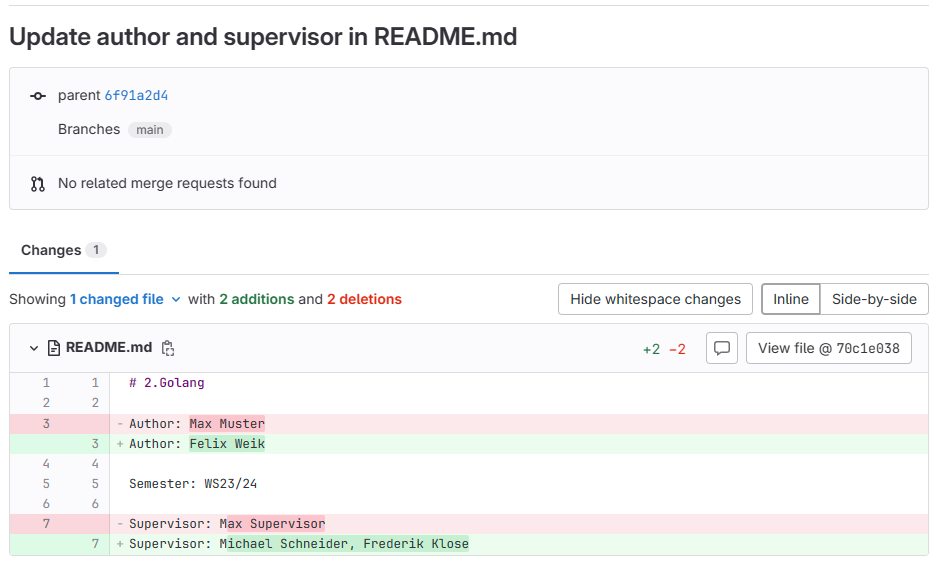
\includegraphics[width=0.8\textwidth]{figures/goLang/golang_screendumpReadmeCommit.png}
    \caption{Screendump showing the Commit Message and the changed Files}
    \label{fig:screendump_readmeCommitMessage}
\end{figure}

\begin{figure}
    \centering
    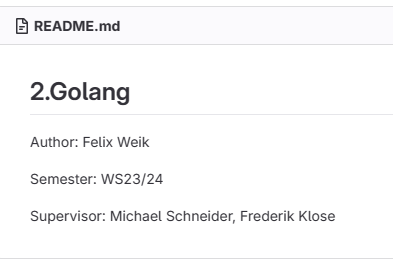
\includegraphics[width=0.5\textwidth]{figures/goLang/golang_screendumpReadme.png}
    \caption{Screendump showing the Updated README.md File}
    \label{fig:screendump_readme}
\end{figure}


%==============================================================================

\section{Basic Go Program HelloWorld}
\label{sec:basic_go_program}
This section implements a simple hello world program, introducing the basic syntax of Golang.

\subsection{Excercise HelloWorld}
\label{sec:excercise_hello_world}
% //TODO Einleitung schreiben
% //TODO Listings style updaten 
\subsubsection*{Run Hello World}
After following the instruction in \cite{MS-GODEV}, the code is executed by running \texttt{go run main.go} in the terminal.
The code was executed twice: The first time the given code was executed leading to the output shown in \autoref{fig:screendump_helloWorld_basicExecution}.
The second time the code was executed with different text, which can be seen in \autoref{fig:screendump_helloWorld_differentText}.

\begin{figure}[H]
    \centering
    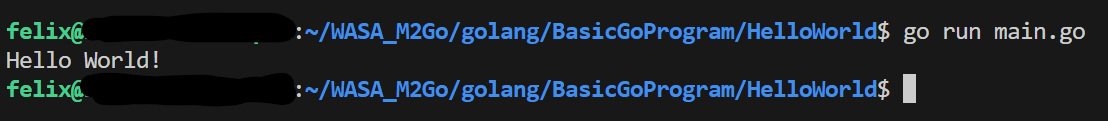
\includegraphics[width=0.8\textwidth]{figures/goLang/helloWorld/golang_helloWorld_basicExecution.png}
    \caption{Screendump showing the basic execution of the Hello World program}
    \label{fig:screendump_helloWorld_basicExecution}
\end{figure}

\begin{figure}[H]
    \centering
    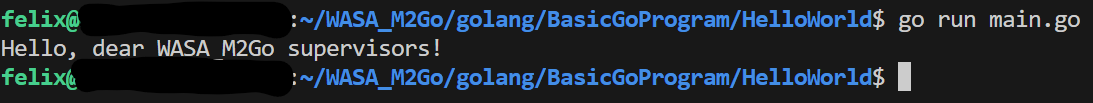
\includegraphics[width=0.8\textwidth]{figures/goLang/helloWorld/golang_helloWorld_ExecutionDifferentText.png}
    \caption{Screendump showing the execution of the Hello World program with different text}
    \label{fig:screendump_helloWorld_differentText}
\end{figure}

\subsubsection*{Code Explanation}
\autoref{lst:helloWorld} shows the code of the Hello World program with explanations of the different parts of the code.
\begin{lstlisting}[
style=kit-cm,
language=Golang,
caption={Hello World Program in Golang with Explanations},
label={lst:helloWorld},
]
// main.go 
// Author: Felix Weik

package main    // package declaration: every executable belongs to the main package
                // by declaring this package, a executable file is produced after compliation

import "fmt"    // import the fmt package, a standard library package 
                // implementing formatted I/O functions
                // after import, one can use the functions of the imported package

func main() {   // declares the function main, which is the 
                // entry point of the program
    fmt.Println("Hello, World!")    // call the Println function 
                                    // of the fmt package; Println prints 
                                    // the given text to the standard output
}               // end of the main function

\end{lstlisting}

\subsubsection*{HelloName}
The goal of this task is to extend the already given HelloWorld program to the HelloName program, prompting the user for a name then showing the given prompt in the output.
The code is shown in \autoref{lst:helloName}:
\begin{lstlisting}[
style=kit-cm,
language=Golang,
caption={Extension of helloWorld to helloName},
label={lst:helloName},
]
// main.go
// Author: Felix Weik

package main

import (
    "fmt"
)

func main() {
    greet()
}

func greet() {
    var name string
    fmt.Print("What is your name? ")
    fmt.Scanln(&name)
    fmt.Println("Hello, " + name + "!")
} 
\end{lstlisting}

The result of the executed code is shown in \autoref{fig:screendump_helloName}

\begin{figure}[H]
    \centering
    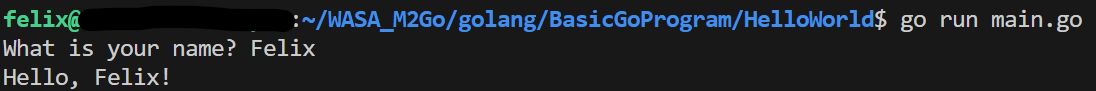
\includegraphics[width=0.8\textwidth]{figures/goLang/helloWorld/golang_helloWorld_helloName.png}
    \caption{Screendump showing the execution of the HelloName program}
    \label{fig:screendump_helloName}
\end{figure}

%==============================================================================

\section{Go Program CarRental}
\label{sec:go_program_car_rental}
%TODO: herausfinden, wie man die autoref namen großschreibt
This section introduces fundamental programming concepts in Golang.
First, the requirements analysis of the CarRental program is conducted, by reviewing an informal story in \autoref{sec:exercise_use_case_diagram_car_rental}.
The following design phase in \autoref{cha:design_of_data_and_functionality} specifies data structures and the functionality of the use case.
The last section introduces concepts of implementing and testing the design artifacts.

\subsection{Excercise UseCaseDiagram CarRental}
\label{sec:exercise_use_case_diagram_car_rental}
The general functionality of the application CarRental is outlined by Alice's Car Rental story as described in \cite{CM-T-GO} listing 3.1.
It provides a general overview of the application and the user flow of registering and renting a car.

By using the story, the use cases and actors can be derived.
The following tasks are based on the story and help derive the use cases, actors and services modeled in the use case diagram.

\subsubsection*{Derive Use Cases and Actors}
The goal of this task is to find four use cases and one actor according to the given story "Alice's Car Rental" from listing 3.1 in \cite{CM-T-GO}.

% //TODO: Herleitung der vier Use Cases beschreiben
\autoref{lst:car_rental_use_case_1} was derived from line 4 of the given story.

In the story Alice rents a car, a VW ID.2, for a certain period.
This is done by entering the rental period and choosing the car from the list of available cars.

After successfully renting the car, the customer is prompted with a rental confirmation and the rental is stored.

\begin{lstlisting}[
    caption={Use Case 1: "Rent a Car"},
    label={lst:car_rental_use_case_1},
    style=kit-cm,
]
Title: Rent a Car
Primary Actor: Customer
Secondary Actor: None

Preconditions:
    - Customer is registered and logged in
    - Customer has a valid driver's license and credit card

Postconditions:
    - Customer has rented a car for the chosen time interval

Flow:
1. The customer calls the application CarRental.
2. The customer enters a start date and end date as the rental period
3. The system shows a list of the cars that are available at the selected rental period
4. The customer selects one of the listed cars
5. The system shows a rental confirmation and stores the rental

Alternative flows:
3a. no cars are available at the selected time interval
    3a1. The system shows a message that no cars are available at the selected time interval and the flow continues from 2 or terminates
4a. The customer does not want to rent any of the offered cars
    4a1. The flow terminates    
\end{lstlisting}

\autoref{lst:car_rental_use_case_2} describes the registration process itself.

It was derived from line 3 of the given story.
In order to use the application, Alice needs to register first.

After successfully registering, Alice can log in to the application and rent a car.

\begin{lstlisting}[
    caption={Use Case 2: "Registering Process"},
    label={lst:car_rental_use_case_2},
    style=kit-cm,
]
Title: Registering Process
Primary Actor: Customer
Secondary Actor: None

Preconditions:
    - The customer is not registered yet
    - Customer has a valid email address
    - Customer has a valid credit card and driver's license
    - Customer is at least 18 years old
    - Customer is not blacklisted by the car rental company or an insurance company

Postconditions:
    - Customer is registered
    - Customer can rent a car
    - Customer can log in to the car rental company's website

Flow:
1. Customer visits the car rental company's website or opens the app 
2. Customer is asked to register or login
3. Customer clicks on "Register"
4. Customer is prompted for email, name, driver's license, credit card number, date of birth
5. A data validation is performed
6. Customer needs to authenticate his email address
7. Customer chooses a password and a username
8. Customer shows a registration confirmation and the customer is registered successfully 

Alternative flows:
3a. Customer is already registered and clicks on "Login" instead of "Register"
5a. Customer prompts false information or leaves nonoptional fields empty, so the data validation fails
    5a1. The customer is asked to fill out the form again
6a. Customer does not authenticate his email address
    6a1. The customer will not be registered and the registration process will be aborted
7a. Customer chooses a username that is already taken
    7a1. The customer is asked to choose another username
7b. The provided password does not fulfill the given criteria
    7b1. The customer is asked to choose a stronger password
\end{lstlisting}

There are two types of cancellation: Cancellation of a rental and cancellation of the registration.
\autoref{lst:car_rental_use_case_3} describes the cancellation of a rental as described in lines 5 and 6 of the given story.

Like Alice in the story, the customer can cancel a rental if he successfully rented a car but does not want to use it anymore.
The customer can cancel the rental as long as the time interval of the rental has not started yet.

After successfully canceling the rental, the customer is prompted with a cancellation confirmation.

\begin{lstlisting}[
    style=kit-cm,
    caption={Use Case 3: "Cancellation of a Rental"},
    label={lst:car_rental_use_case_3},
]
Title: Cancellation of a Rental
Primary Actor: Customer
Secondary Actor: None

Preconditions:
    - Customer has rented a car
    - Customer is logged in
    - The time interval of the rental has not started yet

Postconditions:
    - Customer has cancelled the rental
    - Customer is prompted with a cancellation fee if necessary

Flow:
1. Customer calls the application CarRental
2. Customer clicks on "My Rentals"
3. Customer selects the rental he wants to cancel
4. Customer clicks on "Cancel Rental"
5. Customer is prompted with a cancellation fee if necessary
6. Customer confirms the cancellation
7. Customer is asked to confirm the cancellation again via email
8. Customer confirms the cancellation via email
9. Customer is prompted with a cancellation confirmation

Alternative flows:
3a. Customer has no rentals
    3a1. The system shows a message that the customer has no rentals and the flow terminates
4a. Customer does not want to cancel the rental and the flow terminates
5a. Customer does not want to pay the cancellation fee
    5a1. The flow terminates and the rental is not canceled
8a. Customer does not confirm the cancellation via email
    8a1. The flow terminates and the rental is not canceled
\end{lstlisting}

\autoref{lst:car_rental_use_case_4} describes the cancellation of the registration as described in line 6 of the given story.

In the story, Alice cancels her registration due to personal reasons.
The customer can cancel the registration if he does not want to use the application anymore.

After successfully canceling the registration, the customer is prompted with a cancellation confirmation and can neither log in nor use the application without registering again.

\begin{lstlisting}[
    float=h,
    caption={Use Case 4: "Cancellation of the Registration"},
    label={lst:car_rental_use_case_4},
    style=kit-cm,
]
Title: Cancellation of the Registration
Primary Actor: Customer
Secondary Actor: None

Preconditions:
    - Customer is registered
    - Customer is logged in
    - Customer has no rentals or outstanding payments

Postconditions:
    - Customer is not registered anymore

Flow:
1. Customer calls the application CarRental
2. Customer clicks on "My Account"
3. Customer clicks on "Cancel Registration"
4. Customer confirmes the cancellation
5. Customer is asked to confirm the cancellation again via email
6. Customer confirms the cancellation via email
7. Customer is prompted with a cancellation confirmation

Alternative flows:
3a. Customer has outstanding payments or rentals
    3a1. The system shows a message that the customer has outstanding payments or rentals and the flow terminates
4a. Customer does not want to cancel the registration and the flow terminates
6a. Customer does not confirm the cancellation via email
    6a1. The flow terminates and the registration is not canceled
\end{lstlisting}

\subsection*{Modelling the Use Case Diagram with UMLet}
The installation of the standalone version of UMLet is carried out as follows:
\begin{enumerate}
    \item Download the latest version of UMLet from \url{https://www.umlet.com/changes.htm}
    \item Extract the downloaded archive
    \item Run the executable file \texttt{umlet.sh} in the extracted folder
\end{enumerate}

A screen dump of the folder structure of the extracted archive is shown in \autoref{fig:umlet_folder_structure}.
\begin{figure}
    \centering
    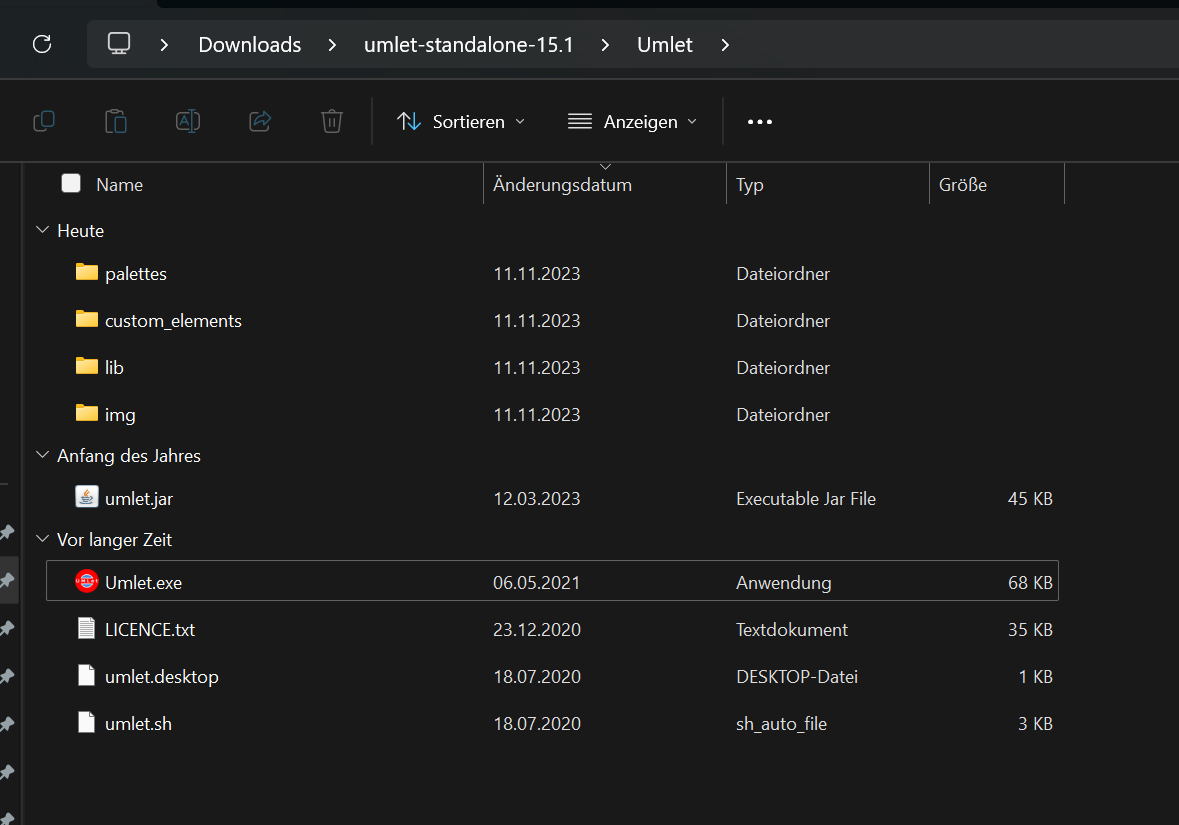
\includegraphics[width=0.8\textwidth]{figures/goLang/carRental/carRental_umletInstallation.png}
    \caption{Folder structure of the extracted UMLet archive}
    \label{fig:umlet_folder_structure}
\end{figure}

The use case diagram is shown in \autoref{fig:car_rental_use_case_diagram}.

It uses so-called services to abstract the implementation of the application.
By providing services, the implementation of the application can be changed without changing the use cases.

The registration service is used to register a customer.
It provides the user interface and structures to interact with the customer.
The registration service itself uses the authentification service to provide the customer with a secure way to authenticate himself, for example by two-factor authentification.
It also uses the cancellation service to cancel the registration if the customer wants to do so.

The rental service is used to rent a car.
It interacts with the location service, providing the location of the customer and the cars and displaying it on a map.
It also uses the cancellation service to cancel the rental if the customer wants to do so.
The car usage service is used to provide the customer with information about the car, for example, if the car is available, the current fuel level or the current mileage.

The services' interactions are displayed in the use case diagram utilizing the arrows and the corresponding labels.
\begin{figure}[H]
    \centering
    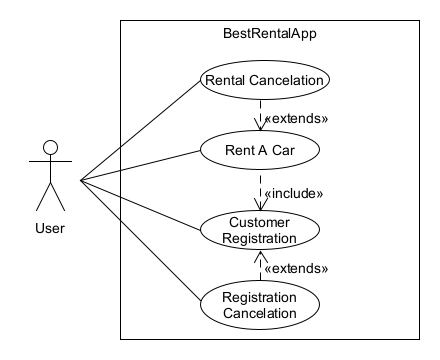
\includegraphics[width=0.8\textwidth]{figures/goLang/carRental/carRental_umlDiagram.png}
    \caption{Use case diagram of the car rental application}
    \label{fig:car_rental_use_case_diagram}
\end{figure}

\subsection{Excercise UseCase RentACar}
\label{sec:exercise_use_case_rent_a_car}
\subsubsection*{Alice's Car Rental}
This task aims to complete the use-case story "Rent a Car" for Alice.
This is done by adding the given data from the story to the use-case story.

The completed use-case story is shown in \autoref{lst:alices_car_rental_use_case_1}.

\begin{lstlisting}[
style=kit-cm,
caption={Alice's Version of Use Case 1},
label={lst:alices_car_rental_use_case_1},
]
1. Alice calls the application CarRental.
2. Alice enters 01.01.00 as a start date and 02.02.00 as the end date as the rental period
3. The system shows a list of the cars that are available at the selected rental period
4. Alice selects a VW ID.2
5. The system shows a rental confirmation and stores the rental

Alternative flows:
3a. The VW ID.2 is not available at the selected time interval
    3a1. The system shows a message that the VW ID.2 is not available at the selected time interval and the flow continues from step 2 or terminates
4a. Alice does not want to rent the VW ID.2
    4a1. The flow terminates
\end{lstlisting}

\label{cha:design_of_data_and_functionality}

\section{Design of the Data and the Functionality}

\subsection{Description of the Initial Entity Diagram}

\subsection{Adding the Attributes}

\subsection{Adding the Functionality as a Method}

\section{Excercise CarRentalStructs}
\label{sec:car_rental_structs}

\subsection*{Add the Attributes to Structs}
After adding the attributes from the entity diagram to the 
\texttt{.../golang/CarRental/CarRentalStructs/CarRentalStructs.go} path and saving
the IDE automatically formats the code and indents it correctly.

\subsection*{Initialize and Print Structs}
The result of the initialization and printing of the structs is shown in figure \ref{fig:car_rental_structs}.
\begin{figure}[H]
    \centering
    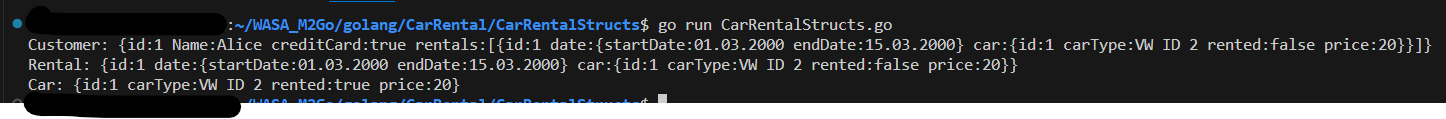
\includegraphics[width=\textwidth]{figures/goLang/carRental/carRental_structs.png}
    \caption{Output of the structs}
    \label{fig:car_rental_structs}
\end{figure}

\subsection*{Create an Array of Rentals}
The function works as follows:
\begin{enumerate}
    \item The array \texttt{cartypes} holds the string of 5 different cartypes
    \item The function \texttt{createRentals(id, date, car)} returns 5 rentals that are appended to the array
    \item Via \texttt{fmt.Println(rentals)} the array is printed into the console
\end{enumerate}

The result looks like this:
\begin{figure}
    \centering
    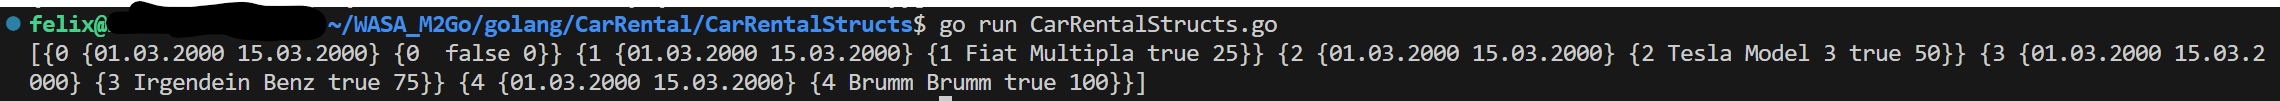
\includegraphics{figures/goLang/carRental/carRental_arrayFiveRentals.png}
    \caption{Output of the Array of Rentals}
    \label{fig:car_rental_array_five_rentals}
\end{figure}


%==============================================================================

\section{Advanced Go Program CarRentalCLI}
\label{sec:advanced_go_program_car_rental_cli}
This section introduces advanced programming concepts in Golang.

The actor needs to input data into the CarRental program to interact with it.
Therefore, CarRentalCLI implements a simple command line interface (CLI) for the CarRental program.

The following tasks will introduce the application by analyzing the software and microarchitecture.
After understanding the program, commands and mappers will be added.
After that, the program will be tested according to a list of OCL constraints.

At the end of this section, further use cases and functionality will be implemented as part of a challenge.

\subsection{Excercise GettingStartedWithCarRentalCLI}
\label{sec:exercise_getting_started_with_car_rental_cli}
This task aims to get familiar with the given code and to understand the structure of the application.

The first task analyzes and completes \autoref{tab:cli_parameters_car_rental_cli}.
Following that, delving into the architecture involves describing and analyzing software and microarchitecture
The last step is to start the program and rent a car for Max.

These tasks will provide a fundamental understanding of the application and its structure.

\subsubsection*{Analyze the CLI Parameters}
The goal of this task is to derive input and output parameters for the CLI commands.
\autoref{tab:cli_parameters_car_rental_cli} is based on the given task sheet and contains the input and output parameters for the CLI commands.

The empty fields are in the spaces where the command, input, and output are not specified in the task sheet.
Empty fields are marked with an underline.

The command for registering as a customer is chosen to be \texttt{register} since it clearly describes the intention and action of the command.

Input for canceling a rental is the \texttt{RentalID}.
This is needed to identify the rental to cancel.
If the cancellation process is successful, the input \texttt{RentalID} is returned.
Else, an error is returned.

The command for deregistering as a customer is \texttt{deregister} since it clearly describes the intention and action of the command.
Only the customer ID is needed as input since it identifies the customer.
If the deregistration is successful, the customer ID is returned to the CLI, showing the value that will be deleted from the YAML file.
If the deregistration fails, the CLI returns a failure message.

The values are shown in \autoref{tab:cli_parameters_car_rental_cli} - newly inserted values are underlined.

\begin{table}[h]
      \centering
      \begin{tabular}{|p{4cm}|p{2cm}|p{4cm}|p{5cm}|}
            \hline
            \textbf{Use Case} & \textbf{Command} & \textbf{Input} & \textbf{Output} \\
            \hline
            \hline
            Register as Customer & \underline{register} & CustomerID, Name & CustomerID / Failure \\
            \hline
            Rent a Car & rent & RentalID, CustomerID, CarID, StartDate, EndDate & RentalID / Failure \\
            \hline
            Cancel Rental & cancel & \underline{RentalID} & RentalID / Failure \\
            \hline
            Deregister as Customer & \underline{deregister} & \underline{CustomerID} & \underline{CustomerID / Failure} \\
            \hline
      \end{tabular}
      \caption{CLI Parameters for CarRentalCLI}
      \label{tab:cli_parameters_car_rental_cli}
\end{table}

\subsubsection*{Describe the Software Architecture}
The provided software architecture is a three-layer architecture consisting of the Presentation Layer, the Application Logic Layer, and the Infrastructure Layer.
Each layer will be explained in the following.

\begin{description}
      \item[CarRentalCLI (Presentation Layer):] 
                  This component handles the user interaction.
                  It uses the \texttt{CarRentalOperationsInterface}.
      \item[CarRentalOperations (Application Logic Layer):]
                  This component implements the \texttt{CarRentalRepositoryInterface} with the CarRentalOperations component.
                  It provides the \texttt{CarRentalOperationsInterface} for the Presentation Layer.
      \item[CarRentalRepository (Infrastructure Layer):]
                  This component is part of the infrastructure layer, ensuring data persistence.
                  The repository therefore is responsible for managing the data from the car rental process providing the according functionality.
\end{description}

\subsubsection*{Analyze the Micro Architecture}
The micro-architecture of an application describes the internal structure of a single subsystem.

\autoref{fig:car_rental_cli_micro_architecture} depicts the micro-architecture built on top of the software architecture.
The focus is the interaction between classes, interfaces and packages within the different layers.

\paragraph*{CLI:}
The \texttt{CarRentalCLI} handles the user interaction.
The class \texttt{CarRentalCLI} implements the cli commands by calling the according functions from the \hfill \linebreak \texttt{CarRentalOperationsInterface}.
This provides a great overview and abstraction, improving the maintainability and scalability of the application.

\paragraph*{Logic:}
This package is responsible for managing the state of the application and for performing the business logic.
The \texttt{CarRentalOperations} class implements the \texttt{CarRentalOperationsInterface} and provides the functions for the \texttt{CarRentalCLI} to call.
The interface hides the infrastructure-specific details and provides a simple interface for the \texttt{CarRentalCLI} to interact with.
Both components share the same model, which is defined in the \texttt{model} subpackage.

\paragraph*{Infrastructure:}
The \texttt{CarRentalRepository} package is responsible for the communication with the YAML files.
It provides the \texttt{CarRentalRepositoryInterface} which is implemented by the \texttt{CarRentalRepository} class.
This class is responsible for storing and retrieving data, hiding the infrastructure-specific calls.
The YAML mappers provide functions to read and write YAML files.
The entities provide the structure of the YAML files and the structure of the struct the mapper creates.
These files represent the database of the application storing the data.

\begin{figure}
      \centering
      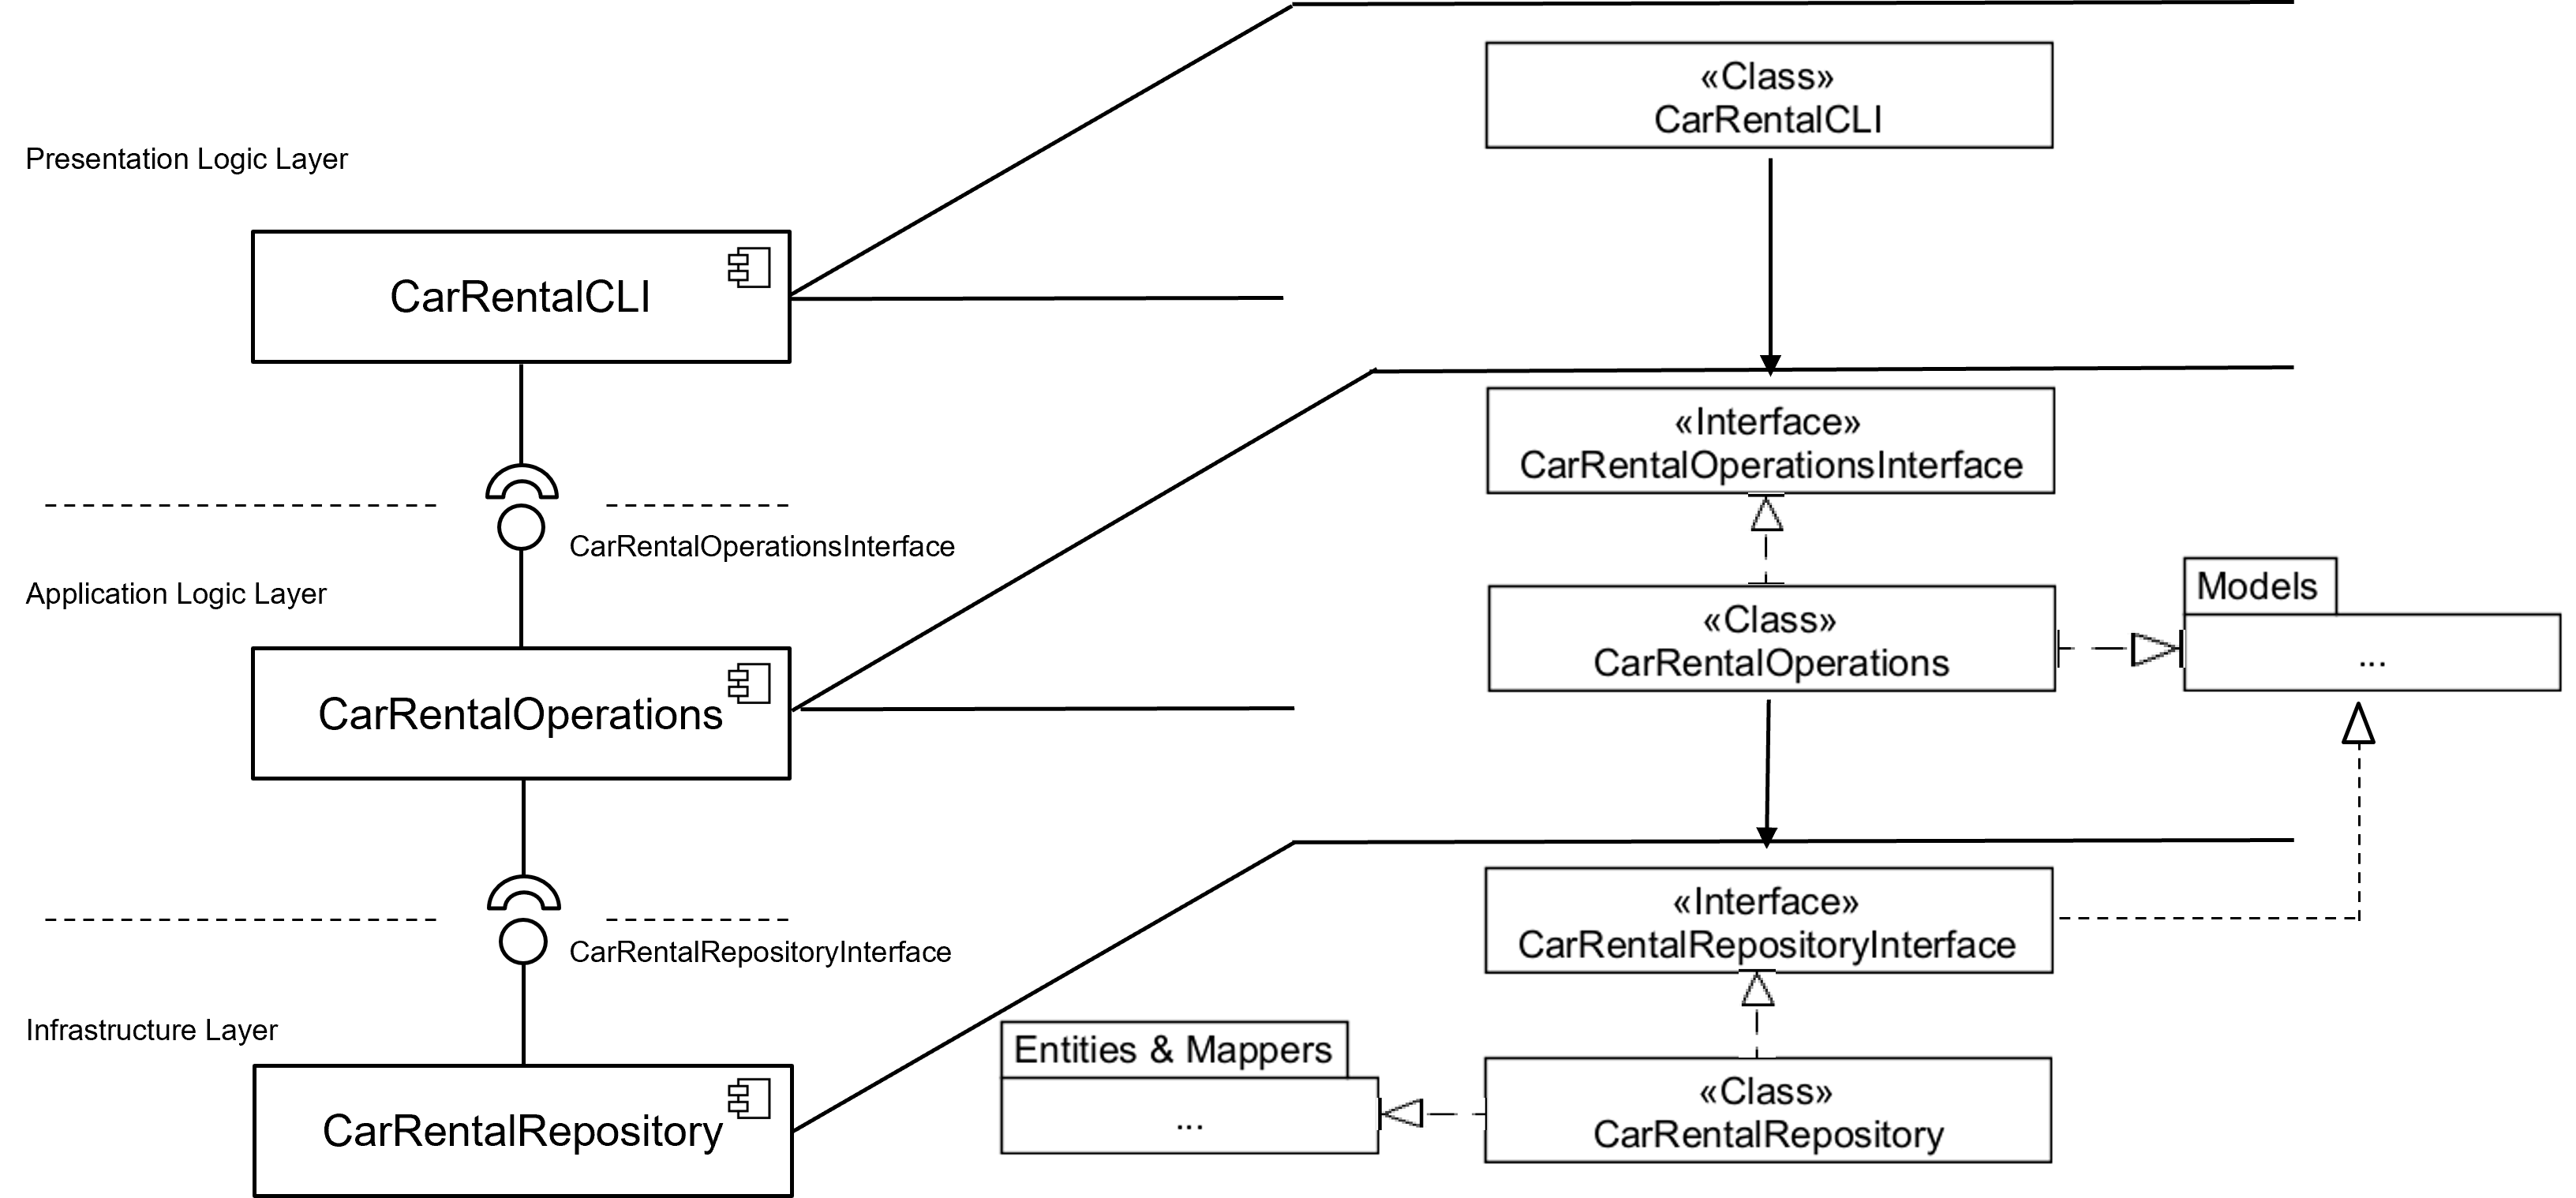
\includegraphics[width=0.8\textwidth]{figures/goLang/carRental/carRentalCLI/carRentalCLI_MicroArchitecture.png}
      \caption{Micro Architecture of the CarRentalCLI}
      \label{fig:car_rental_cli_micro_architecture}
\end{figure}

\subsubsection*{Start the Go Program CarRentalCLI}
The program can be started by running \texttt{go run main.go <command>}.
To rent a car \texttt{go run . --- rent} is executed in the \texttt{./CarRentalCLI} directory.

The program asks for the ID of the customer and the ID of the car.
After entering the IDs, the program asks for the start and end date of the rental by asking for the day, month and year.
If the data is entered correctly and the rental is successful, the program prints a success message and exits.
Otherwise, the program asks for the remaining data and prints an error message, the exit status and exits.

The successful execution of the program is displayed in \autoref{fig:car_rental_cli_successful_rental_max}.

\begin{figure}
      \centering
      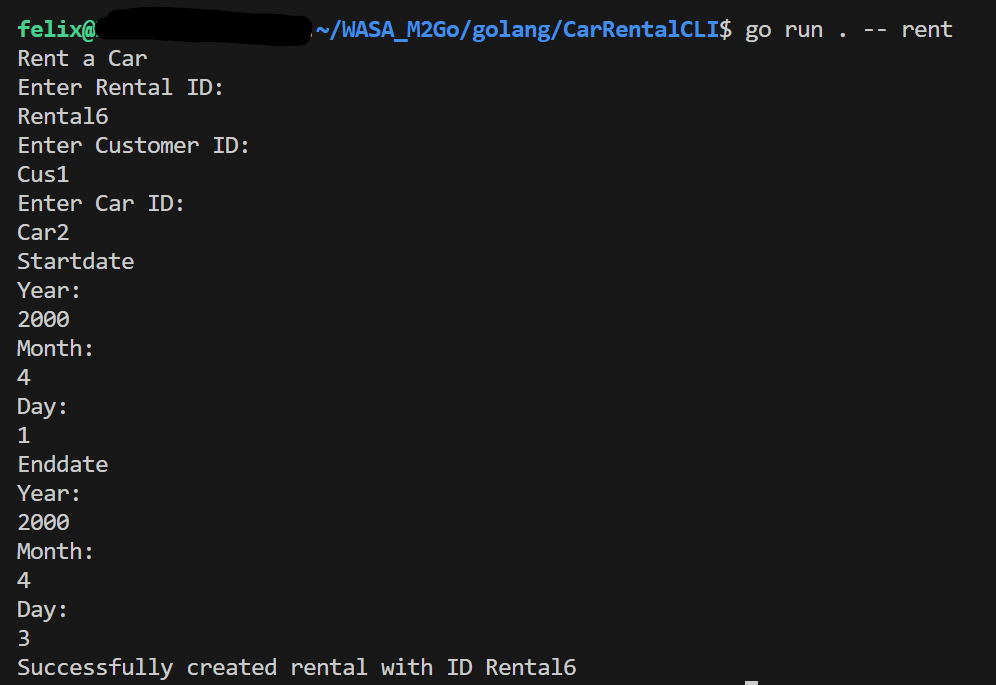
\includegraphics[width=0.8\textwidth]{figures/goLang/carRental/carRentalCLI/carRentalCli_SuccessfulRentalMax.png}
      \caption{Successful Rental of a Car for Max}
      \label{fig:car_rental_cli_successful_rental_max}
\end{figure}

\subsection{Excercise AddRegisterAsCustomer}
\label{sec:exercise_add_register_as_customer}
This task adds the functionality to register as a customer.

To fulfill this task, the following steps are required:
First, a CLI command is added to the presentation layer which calls the basic functions to register a new customer.
After that, an entity mapper is added to the infrastructure layer.
Then, the operation is implemented including validations.
The last step is to test the functionality by registering Alice as a customer.

\subsubsection*{Add CLI Command}
The CLI commands are placed in the \texttt{CarRentalCLI.go} file.
The \texttt{NewCarRentalCLI} function takes \texttt{operations.CarRentalOperations} as input and returns a \texttt{CarRentalCLI} object that can be executed.
This function also specifies the commands that can be executed by the CLI.
The array \texttt{Commands} contains these commands consisting of the name, the usage, and the according action.

To add the command for registering a new customer, the array \texttt{Commands} is extended by the command \texttt{register} with the usage \texttt{Register as Customer}.
The action defines a function taking a CLI-context object as input and returning an error.
This function calls the according function that executes the code executing the actual task.

The code for the new CLI command \texttt{register} is shown in \autoref{lst:car_rental_cli_command_register}.
The new customer is created in \autoref{lst:car_rental_cli_create_customer_persistence_entity}.

\begin{lstlisting}[
      float=h,
      style=kit-cm,
      caption={Code for the CLI Command "register"},
      label={lst:car_rental_cli_command_register},
      language=Golang
]
...
// array and function definition
... // other commands
{
      Name:  "register",
      Usage: "Register as Customer",
      Action: func(cCtx *cli.Context) error {
            return RegisterAsCustomerAction(operations)
      },
},
... // other commands
\end{lstlisting}

\begin{lstlisting}[
      float=h,
      style=kit-cm,
      caption={Creating a Customer Persistence Entity},
      label={lst:car_rental_cli_create_customer_persistence_entity},
      language=Golang
]
// file: CarRentalRepository.go
...
func (repository CarRentalRepository) CreateCustomer(customer model.Customer) error {
	var newCustomer = YAMLMapper.ConvertCustomerToCustomerPersistenceEntity(customer)

	repository.Customers = append(repository.Customers, newCustomer)
	repository.SaveData()
	return nil
}
...
\end{lstlisting}

\subsubsection*{Add Entity Mapper}
What is the necessity for a mapper?
The general task of a mapper is to enable communication between the application and the database.
In this case, the database is a YAML file.
Therefore the mapper can read and write to the YAML files and convert the data to the corresponding entities and vice versa.

Also, mappers are important in terms of decoupling.
They give the possibility to switch the infrastructure layer by adjusting the mappers only.

In the use case of registering a new customer, the mapper is called while creating a new customer.
This mapper is located in the \texttt{./CustomerMapper.go} file, containing two functions.
The first function \texttt{ConvertCustomerToCustomerPersistenceEntity} takes a customer object as an argument and returns a customer persistence entity containing the same values.
This entity is then written to the YAML file.
By writing the entity into the YAML file, the customer is registered and can be used in the application.

The second function \texttt{ConvertCustomerPersistenceEntityToCustomer} takes a customer persistence entity as an argument and returns a customer object containing the same values.
It acts just like the function above but in the opposite direction.

This task is about implementing the \texttt{ConvertCustomerToCustomerPersistenceEntity} function.
The code for this function is shown in \autoref{lst:car_rental_cli_mapper_customer_to_customer_persistence_entity}.

\begin{lstlisting}[
      float=h,
      style=kit-cm,
      language=Golang,
      caption={Code for the ConvertCustomerToCustomerPersistenceEntity Function},
      label={lst:car_rental_cli_mapper_customer_to_customer_persistence_entity},
]
// CustomerMapper.go
// author = Felix Weik

func ConvertCustomerToCustomerPersistenceEntity(customer model.Customer) entities.CustomerPersistenceEntity {
return entities.CustomerPersistenceEntity{
      ID:   customer.ID,
      Name: customer.Name,
}
}
\end{lstlisting}

\subsubsection*{Implement Operation}
The registering process is implemented in separate files across the different layers.

The CLI command "register" calls the \texttt{RegisterAsCustomerAction} function starting from the \texttt{CarRentalCLI.go} file.
This function is located in the \texttt{CliActions.go} file.
It prints a message to the CLI and collects the customerID and the customerName attributes via other functions from the CLI package.

After that, it calls the \texttt{RegisterAsCustomer} function that takes both collected \hfill \linebreak values as input.
This function is located in the operations package in the \hfill \linebreak \texttt{RegisterAsCustomerOperation.go} file.
It validates the input by checking if the customer exists.
If the input is valid, it calls the \texttt{NewCustomer} and \texttt{CreateCustomer} functions, which are located in the models package.
These functions will write to the YAML file, storing the new customer.

If an error occurs or the validations fail, the process will abort.
If the process succeeds, a success message containing the newly created customer ID is printed to the CLI.

\subsubsection*{Register Alice as Customer}
After running the CLI command to register a new customer, the program asks for the ID of the customer.
In this case, Alice receives the ID \texttt{Cus5}.
After entering the ID, the program asks for the name of the customer, in this case Alice.
The program exits with a success message and the exit status as shown in \autoref{fig:car_rental_cli_register_alice}.

To register a new rental, the program starts with \texttt{go run . --- rent}.
The program asks for the ID of the rental, here it is \texttt{Rental7}.
The customer ID for Alice is \texttt{Cus5}.
After that, the start and end date is entered.
The program exits with a success message and the exit status as shown in \autoref{fig:car_rental_cli_rental_alice_successful}.

\begin{figure}
      \centering
      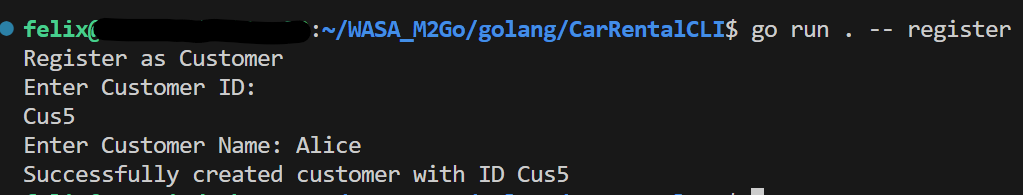
\includegraphics[width=0.8\textwidth]{figures/goLang/carRental/carRentalCLI/carRentalCLI_RegisterAlice.png}
      \caption{Register Alice as a Customer}
      \label{fig:car_rental_cli_register_alice}
\end{figure}
\begin{figure}
      \centering
      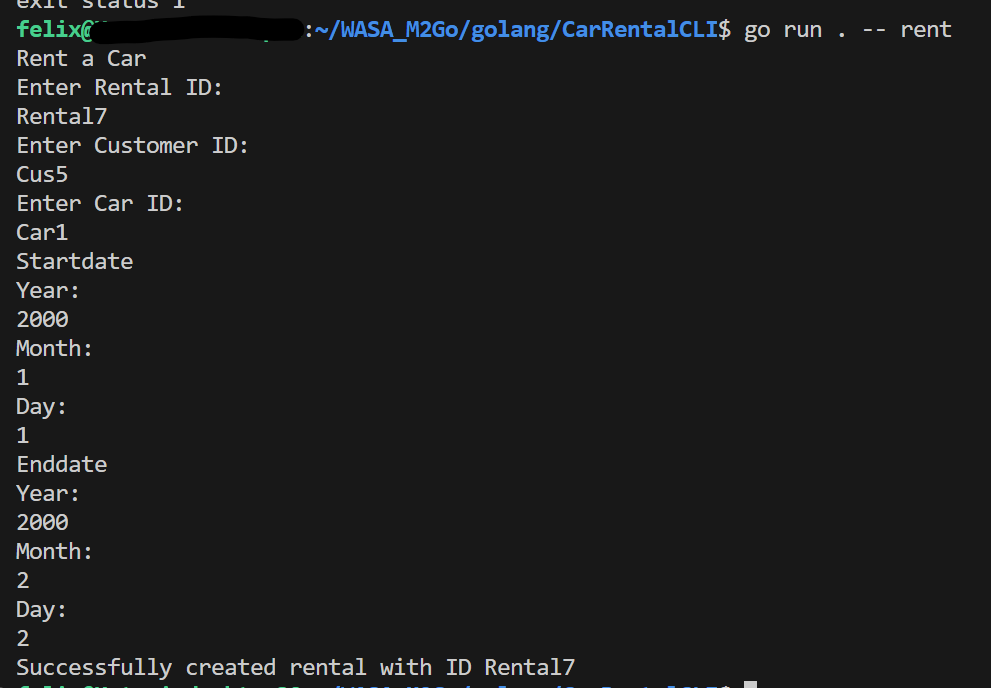
\includegraphics[width=0.8\textwidth]{figures/goLang/carRental/carRentalCLI/carRentalCLI_SuccessfulRentalAlice.png}
      \caption{Successful Rental of a Car for Alice}
      \label{fig:car_rental_cli_rental_alice_successful}
\end{figure}

\subsection{Excercise TestCarRentalCLI}
\label{sec:exercise_test_car_rental_cli}

\subsubsection*{Derive Test Cases}
For the sake of simplicity, we asume that a correct car called \texttt{correctCar} and customer called \texttt{correctCustomer} are provided.
In the cases where the date is correct we assume the date \texttt{startDate} and \texttt{endDate} represent correct dates.
In our case we assume the startDate to be the 01.01.2000 and the endDate to be the 02.02.2000.

First we define positive and negative test cases for the \texttt{NewRental} function.
\begin{lstlisting}[
    language=Golang,
    caption={Test Cases for the Rental Context},
    label={lstlisting:rental_test_cases},
    numbers=left,
    numberstyle=\tiny
    ]
    // Constraint 1: self.ID -> notEmpty()
    NewRental("", startDate, endDate, correctCar, correctCustomer) // negative test case
    NewRental("Rental1", startDate, endDate, correctCar, correctCustomer) // positive test case

    // Constraint 2: self.startDate -> notEmty()
    NewRental("Rental2", date{}, endDate, correctCar, correctCustomer) // negative test case
    NewRental("Rental2", startDate, endDate, correctCar, correctCustomer) // positive test case

    // Constraint 3: self.endDate -> notEmty()
    NewRental("Rental3", startDate, date{}, correctCar, correctCustomer) // negative test case
    NewRental("Rental3", startDate, endDate, correctCar, correctCustomer) // positive test case

    // Constraint 4: self.startDate < self.endDate
    NewRental("Rental4", endDate, startDate, correctCar, correctCustomer) // negative test case
    NewRental("Rental4", startDate, endDate, correctCar, correctCustomer) // positive test case

    // Constraint 5: self.car -> notEmpty()
    NewRental("Rental5", startDate, endDate, car{}, correctCustomer) // negative test case
    NewRental("Rental5", startDate, endDate, correctCar, correctCustomer) // positive test case

    // Constraint 6: self.customer -> notEmpty()
    NewRental("Rental6", startDate, endDate, correctCar, customer{}) // negative test case
    NewRental("Rental6", startDate, endDate, correctCar, correctCustomer) // positive test case
\end{lstlisting}
  
Now, we define positive and negative test cases for the \texttt{rentACar\(\)} function.
This function takes the rentalID, start and endDate, the car, and the customer as arguments.
If the function is executed correctly it will return the new rental.
We specified in the beginning of the section, startDate, endDate, correctCar, and correctCustomer represent correct parameters.

\begin{lstlisting}[
    language=Golang,
    caption={Test Cases for the Rental Context},
    label={lstlisting:rental_test_cases},
    numbers=left,
    numberstyle=\tiny
    ]
    // Constraint 1: pre: self.rentalID -> not exists
    rentACar("Rental1", startDate, endDate, correctCar, correctCustomer)
    rentACar("Rental1", startDate, endDate, correctCar, correctCustomer) // negative test case due to function executing twice
    rentACar("Rental2", startDate, endDate, correctCar, correctCustomer) // positive test case

    // Constraint 2: and Rental.allInstances() -> 
    //  forAll(r: Rental | r.car = self.car implies(self.endDate < r.endDate or r.Endate > self.startDate))
    rentACar("Rental3", startDate, endDate, correctCar, correctCustomer)
    rentACar("Rental4", startDate', endDate, correctCar, correctCustomer') // negative test case due to overlapping dates for the same car
    rentACar("Rental5", startDate', endDate', correctCar, correctCustomer') // positive test case 

    // Constraint 3: post: self.rentals -> includes(rental)
    rentACar("Rental6", startDate, endDate, correctCar, correctCustomer) // positive test case
    rentACar("Rental7", date{}, endDate, correctCar, correctCustomer) // negative test case => due to constraint 2, the element will not be created and therefore will not appear in the list
    
\end{lstlisting}

\subsubsection*{Analyze Test Structure}
% Structure description of the test file and mock-repository
The MockCarRepository acts similar to the actual CarRepository.
It implements the CarRentalRepositoryInterface and provides the according functions.
Furthermore, it also implements the lists of the models \texttt{Rental}, \texttt{Car}, and \texttt{Customer}.
However, there is no constructor and no manipulation of yaml files.
All data-manipulations are done in the memory of the mock-repository.
Therefore the mock-repository only imports the used models.

The test file \texttt{RentACarOperation\_test.go} implements the tests for the \texttt{RentACar} function.
It creates the testint environment by implementing the constructor of the mock-repository, populating it with test data.
After the setup the executable tests are implemented.

% Structure description of the test function TestCarRentalOperations_RentACar
The implementation of the tests happens in the \texttt{TestCarRentalOperations\_RentACar} function.
The \texttt{fields} struct defines the repository used in each test and therefore the test environment.
After that, the \texttt{args} struct defines the arguments needed for the \texttt{RentACar} function.
Now, the test cases are implemented containing the following values:
\begin{itemize}
      \item fields: The repository used in the test as specified above
      \item name: The name of the test
      \item args: The arguments for the \texttt{RentACar} function as specified above
      \item want: The expected return value of the \texttt{RentACar} function, in this case a String 
      \item wantErr: True, if an error is expected, false otherwise. 
            This allows the implementation of negative test cases without the tests failing.
\end{itemize}

% Differences between the mock and the normal repository
The following differences occur between the mock and the normal repository:
\begin{itemize}
      \item The mock repository does not implement a constructor
      \item The mock repository does not manipulate any yaml files, everything is done in the mock repository's lists.
      \item The mock repository only imports the models used in the tests.
      \item The mock repository is only used for testing while the normal repository is used in the application.
      \item The mock repository is located in the same package as the test file (operations), while the normal repository is located in the infrastructure package.
\end{itemize}

However, there are still some similarities:
\begin{itemize}
      \item Both repositories implement the CarRentalRepositoryInterface and therefore provide the same functions.
      \item The provided functionalities are somewhat similar besides the differences mentioned above.
      \item Both repositories are adressed via an operations object representing the repository
\end{itemize}

% Why is a mocked repository required?
Now, why is mocked repository required?
First of all, the mock repository is required to test the functionality of the \texttt{RentACar} function.
This could also be done with the normal repository, however, this would require the manipulation of the yaml files, which arises the following problems:
\begin{itemize}
      \item Test data and actual application data are mixed up
      \item The test data is not reset after the test, which could lead to problems in the next test
      \item The test data needs no be cleaned up after the test, which is not necessary with the mock repository
      \item By creating a certain testing environment, the testing data can manipulated to test the wanted scenarios
\end{itemize}

Further benefits and the actual usage and implementation of both the normal and the mock repository are further explained in \ref{sec:go_repositories}.

\subsection*{Run Tests}

\section{Challenge: Final Use Cases and Further Functionality}
\label{sec:challenge_final_use_cases_and_further_functionality}

\subsection{Challenge AddMissingFunctionalitiesToCarRentalCLI}
\label{subsec:challenge_addmissingfunctionalitiestocarrentalcli}

\subsubsection*{Implement Use Cases}
Two use cases are missing in the CarRentalCLI program.

The first use case is to cancel an already existing rental.

The implementation process is quite similar to the already implemented use cases.
\texttt{CarRentalCLI.go} holds the CLI commands.
By adding "cancel" to the commands array, the command can be used in the CLI.
The command calls the \texttt{CancelRentalAction} function, taking the operations as input.

\texttt{CancelRentalAction} prints "Cancel a rental" and collects the rentalID from the user.
The rental is then canceled by calling \texttt{CancelRental}, taking the rentalID as input.

\texttt{CancelRental} verifies the rentalID by checking if it exists. \hfill \linebreak
It then calls \texttt{DeleteRental(rentalID)} to delete the rental.
The \texttt{DeleteRental} function located in the repository removes the rental from the repository, then saves the data to the yaml files.

If everything runs successfully, a success message is printed to the user containing the removed rental ID.
If an error happens during runtime, the application exits safely.

To test the function, a new file called \texttt{CancelRentalOperation\_test.go} is created.
It uses the already implemented \texttt{SetupMockCarRentalRepository} function from \hfill \linebreak \texttt{CarRentalRepository\_test.go} to create a mock repository.

The function running the tests is similar to the already implemented test function from \texttt{CarRentalRepository\_test.go} besides the test cases.
The test cases only contain the rental ID as a parameter, since it is the only input needed to delete a rental.

Two test cases are implemented:
The first test case is nonconflicting and deletes the already existing first rental.
The second test case is built to fail by wanting to delete a non-existing rental.

Both tests succeed as shown in \autoref{fig:carRentalCLI_challenge_successfulCancellationOfRentalTest}.

\begin{figure}
    \centering
    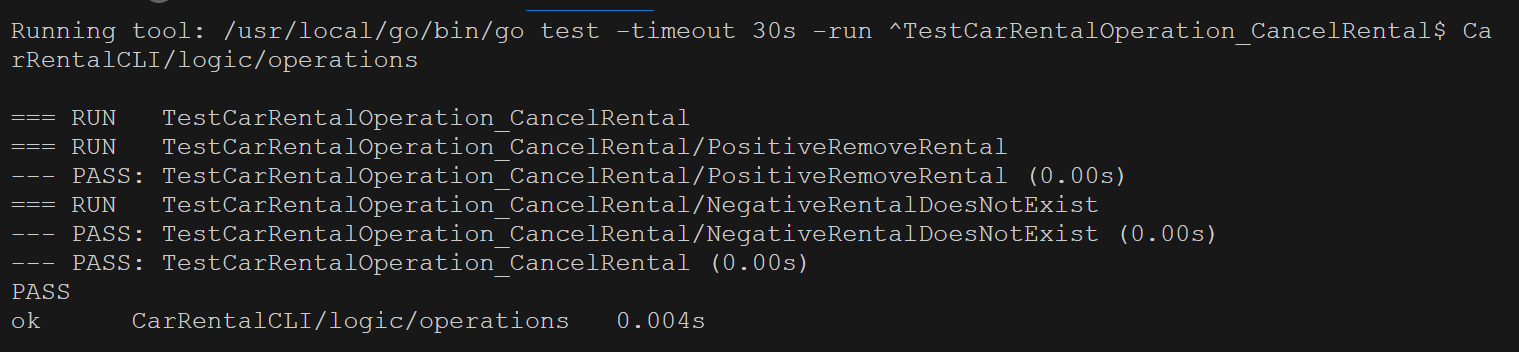
\includegraphics[width=0.8\textwidth]{figures/goLang/carRental/carRentalCLI/challenge/carRentalCLI_challenge_successfulCancellationOfRentalTest.png}
    \caption{Successful Tests of the Newly Implemented CancelRental Function}
    \label{fig:carRentalCLI_challenge_successfulCancellationOfRentalTest}
\end{figure}


%==============================================================================